\documentclass[11pt]{article}

\usepackage[top = 2cm, bottom = 2cm, right = 2cm, left = 2cm]{geometry}

\usepackage{hyperref}
\usepackage{graphicx}
\usepackage{bm}
\usepackage{amssymb}

\begin{document}

\begin{itemize}
    \item HMM profile can be created with hhmake after computing the alignment with hhblits. However it does not work well if the alignment is too diverse (high neff)
    
    \item \textbf{!!! When using plmC, it is super important to add the '-f' flag which specifies the target sequence. Otherwise the results are going to be wrong!!!}
    
    \item March 18, Week 12
    PSI-Blast can compute the PSSM. Both AlphaFold and ProSPr used it. Here is how to use it (it can be installed from conda: conda install -c bioconda blast):
    
    \href{https://www.ncbi.nlm.nih.gov/Class/Structure/pssm/pssm_viewer.cgi}{PSSM viewer link}
    
    And here is how to use HHblits
    
    
    
    I created functions for generating padded crops of given size. The final function takes an input of size (channels, L, L) and output (L, L) and creates batches of size "c" (64 in case of Alphafold). => input (batch, channels, c, c) and output (batch, c, c). For proteins that are shorter than "c", their matrix is places at random offset inside a zero matrix of size (c, c). Proteins, for which length equals k*L, can be cropped two ways. Either with $(k)$ crops (resulting in no zero padding) or $(k+1)^2$ crops (resulting in maximum zero padding). The choice depends on the random state of the system (either even or odd number). For larger proteins a cropping scheme with $k = L // 64 + 1)^2$ crops is created. The crops are randomly offsetted (with the restriction of fitting into the padded area - max allowed padding is c // 2).
    
    \item March 04, Week 10 - \textbf{Understanding Input}
    Today I installed the HH-Suite, which contains the HHBlits algorithm. I also installed MMSeqs2 for sequence search.
    
    \textbf{PLMC}
    
    Tool for generating Potts model. By adding flag \texttt{-c <couplings\_file>} we get a file with Frobenius Norms of the J matrix.
    \item February 22, Week 8
    
    Today I created the AlphaFold network together with the training function. So far the training function does not work with crops but for every domain in an epoch, it randomly selects pairs of indices and creates batches of indices. For each particular batch, there could be a function that loads the desired input and output data, so that the input would have shape = (batch size, input layer size, input dim, input dim), eg (32*32, 613, 32, 32). (32*32 is the size of randomly chosen indices, to imitate the size of crop)
    
    Then on these batches we can perform SGD. The creation of batches is there only for the reason of avoiding loading data for every aminoacid pair for every iteration.
    
    After we loop through all domains, it is time to compute the  training error and validation. In order for it to not take too much time, we can randomly pick few domains from the train\_domains list and val\_domains list, and for each such domain create a random batch of indices and calculate the error. This is still in progress and does not work yet.

    \item February 21, Week 8
    
    \begin{Large}
    \textbf{Input}
    \end{Large}

    We need to make sure that we take into account also context around the desired aminoacid pair. The way ProSPr did it is shown in figure below:
    
    \begin{center}
        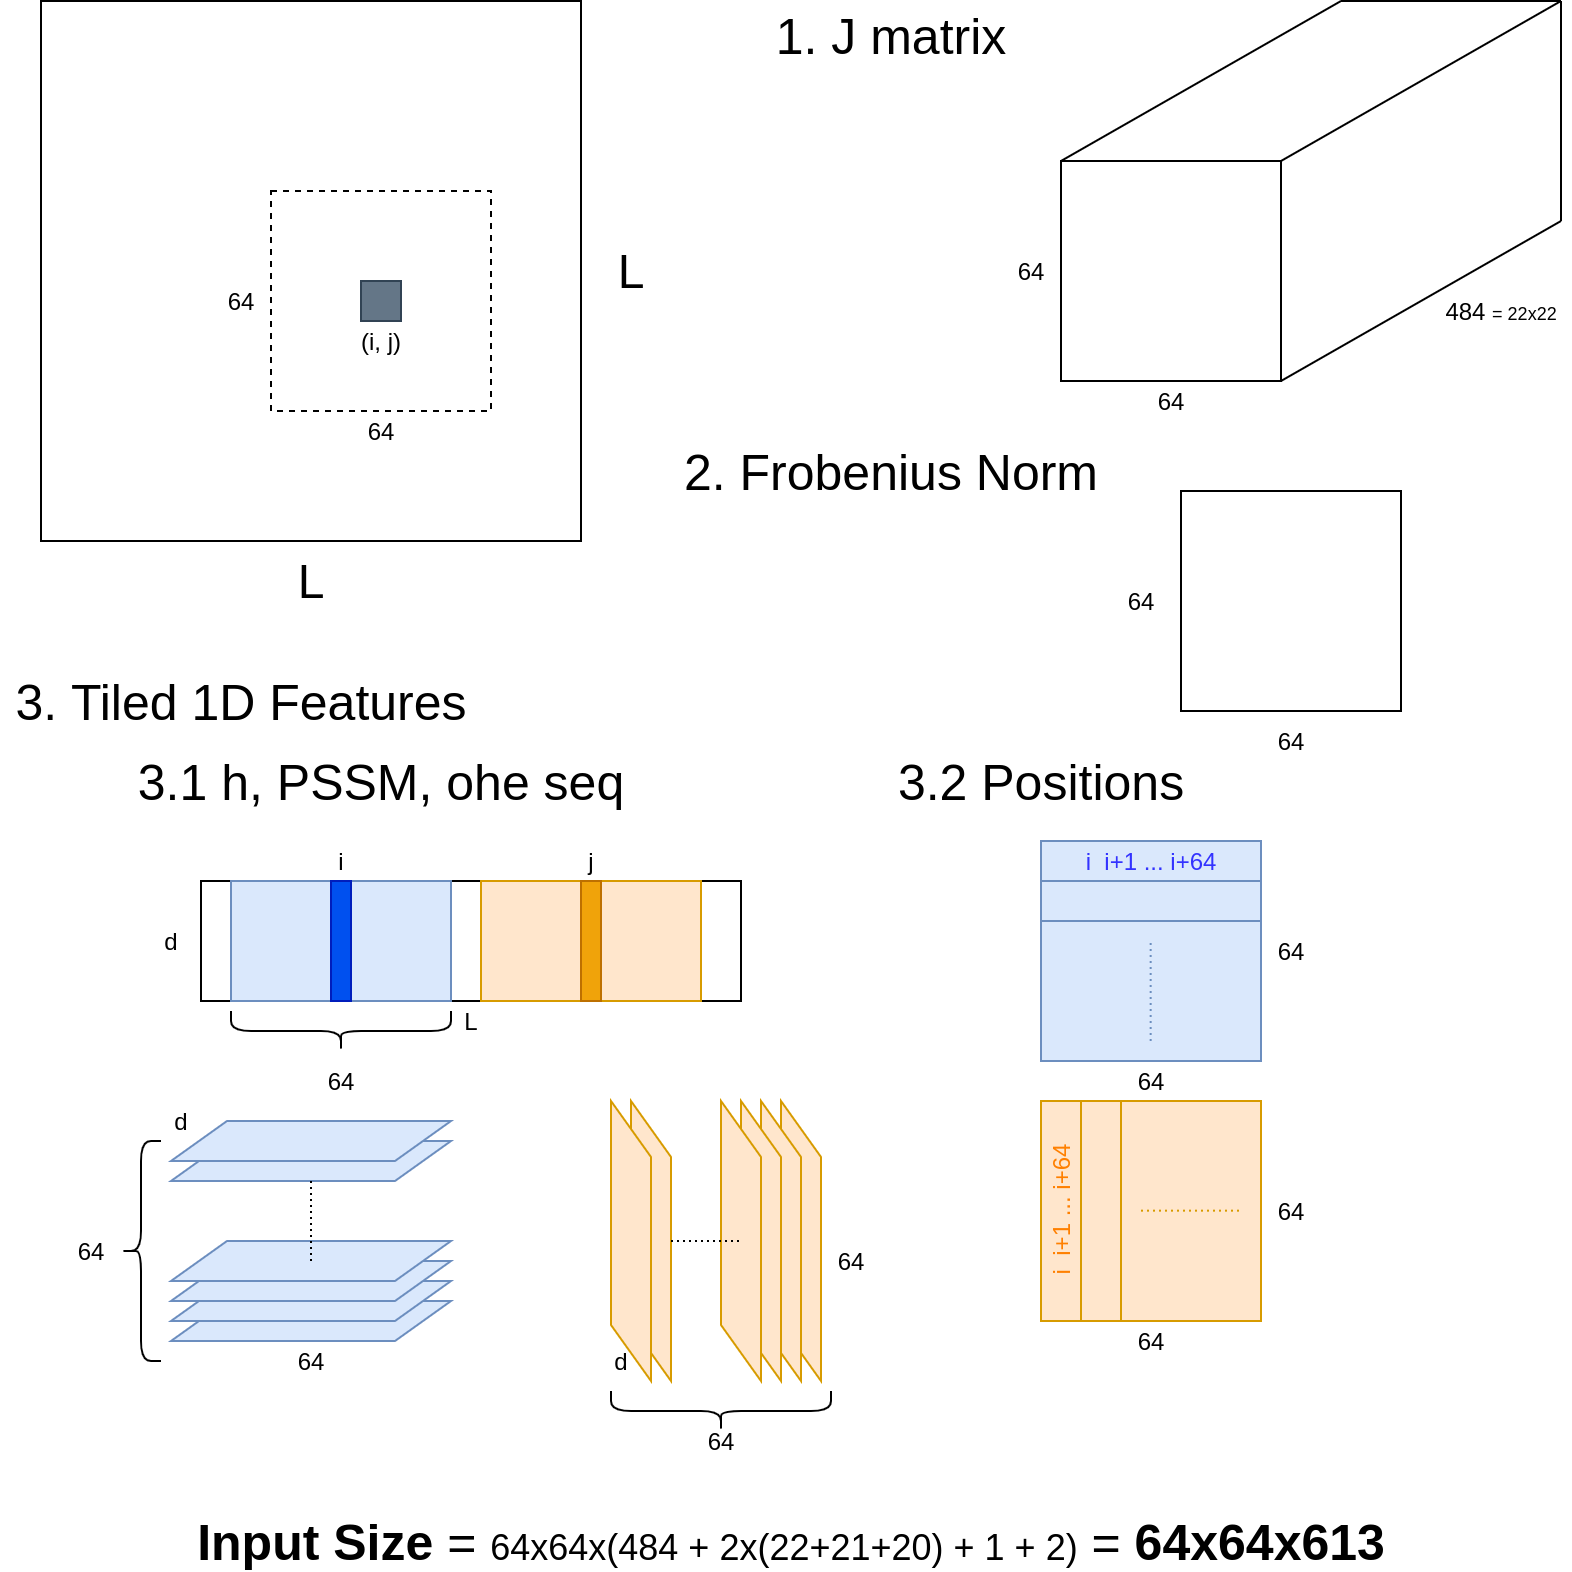
\includegraphics[scale = .25]{imgs_tomas/input_diagram.png}
    \end{center}

    \item February 15, Week 7
    
    - Why does it make sense to use Potts models - especially why should we care about the values of other amino acid pairs in the frobenius norm matrix? 
    
    We are actually going to use a 22x22 matrix from the J variable together with a value from frobenius norm and columns from h matrix and PSSM
    
    \begin{center}
        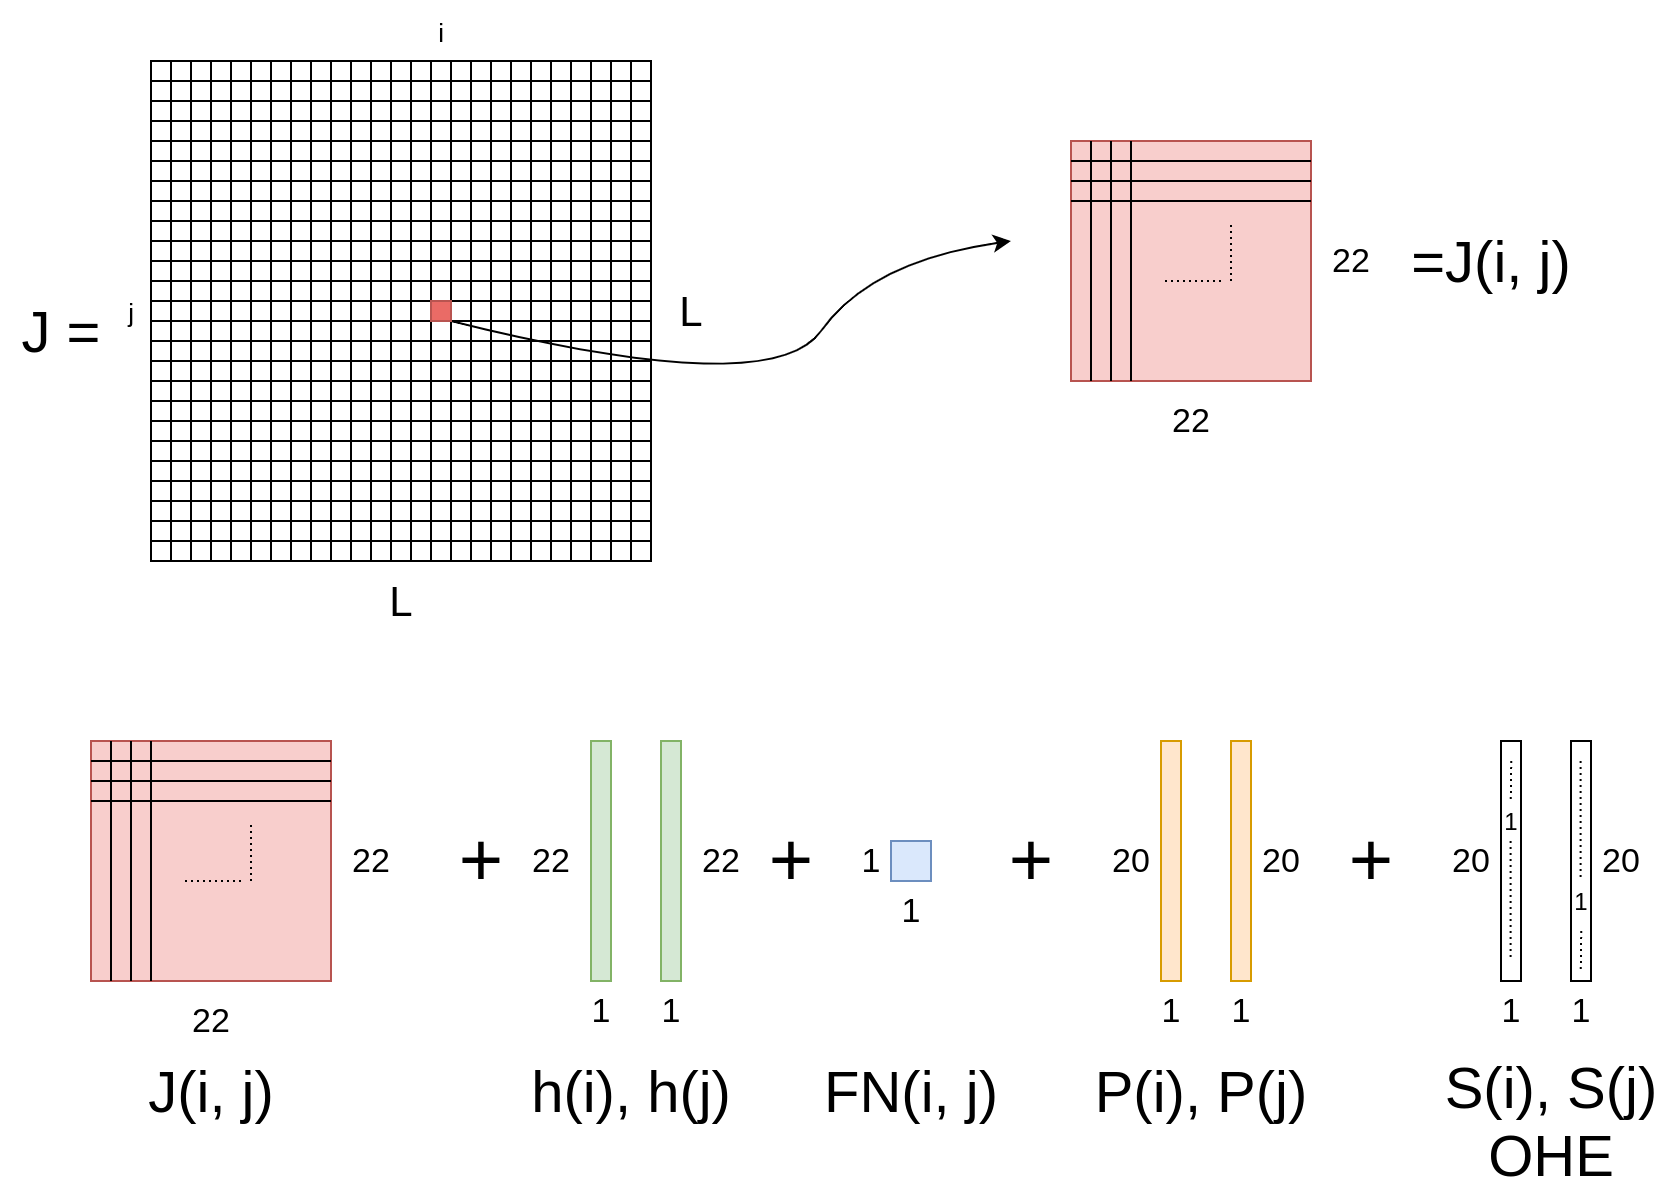
\includegraphics[scale = 0.2]{imgs_tomas/input_features.png}
    \end{center}
    
    - Should we have a neuron for predicting missing values in the last layer?
    
    \item February 06, Week 6
    
    The last few days were not really neccessary, because as it turns out ProSPr offers (on top of the Potts models) the PSSMs, sequences (with gaps denoted with `-`), distance bins for every domain, train, test and validation splits, torsion angles ($\Phi, \Psi$), and others such as the HHblits profile and something called SS.
    
    Short description of the input is included below
    
    \begin{itemize}
        \item \textbf{Potts models} (already described below from February 3)
        
        \begin{itemize}
            \item \textit{Frobenius Norm of $\bm{J}$} (LxL)
            \item \textit{$\bm{h}$} (Lx22) - WHY 22???
        \end{itemize}
        \item \textbf{PSSMs} (Position Specific Substitution Matrices)
        
            PSSMs are very simple statistics of MSA. They describe the occurence of each symbol in our alphabet at each position of the matrix. Lets assume that the alphabet $\bm{\mathcal{A}}$ is of size $N$ and protein is of size $L$. To get the PSSM, one has to follow these steps:
            \begin{enumerate}
                \item Define a position probability matrix $\bm{\mathcal{M}} = \{m_{ij}\}$ (LxN) where:
                $$m_{ij} = \frac{1}{N} \sum_{j = 1}^{N} I(X_{ij} = \bm{\mathcal{A}_j})$$
            
                \item PSSM ($\bm{\mathcal{P}} = \{p_{ij}\})$ is then calculated as:
                $$p_{ij} = log_2\left(\frac{m_{ij}}{b_j}\right)$$
            \end{enumerate}    
                where $b_j$ is the prior probability of a symbol.
                
                An interesting property of PSSMs is, that if one wants to know the likelihood of a sequence, he can sum the log-likelihoods for the particular symbols at the positions. In practice values larger than 1 mean that the sequence is conserved and likely is responsible for some function. If it is less than zero, than it is probably random.
                
                The dimensionality of a PSSM is simply (Lx20) (for aminoacids).
        \item \textbf{HHblits profile} (Lx30)
        
        
        \item \textbf{SS} (Lx1) 
    \end{itemize}
    
    \item February 05, Week 6
    
    I removed 2 domains from the train dataset, because Biopython had troubles openning them - `2me8A00` and `3cmyA00`

    \item February 04, Week 6
    
    The plan for today is to generate output from the PDB files. They are all downloaded. Now the problem is, that PDB files only contain atoms for which the coordinates are known. Thus there might be parts of domains not included in the PDB files. The guys from ProSPr did not care, and they simply made the potts models only from the known atoms. This means that a domain of size 100, might have potts model, eg. the $\bm{h}$ matrix of dimensions $90 \times 22$. I think that we should fix this, by adding rows of zeros, or some other constant so that the spatial effect is conserved. But I am not really sure.
    
    OOkay...
    
    So I needed to make adjustments to take into account some weirdness happenning in few of the domains. But it seems like its working now.
    
    \textbf{ALSO} I removed domains with domain id == '0'. There were only 3 such domains, and I was lazy to fix them

    \item February 03, Week 6
    
    \textbf{The Ising Model}
    
    The entire DCA/Potts models are based on a theory from ferromagnetism called Ising model. 
    
    Lets imagine that we have a 1 dimensional system of magnets. Each one of them can either point up or down - which we can call a spin/magnetization of a magnet. An example with one possible magnetization configuration is shown in the figure below.
    
    \begin{center}
        \includegraphics[scale = 0.5]{imgs_tomas/ising.png}
    \end{center}
    
    Value of each magnet - $\sigma_i$ can be either $+1$ or $-1$. The interaction between two magnets is represented by a variable $\mu_i = \sigma_i \cdot \sigma_{i+1}$. This means that if two magnets point to the same direction, their product will be one. Otherwise it will be $-1$.
    
    Now the question: Lets assume that one particular spin at postion $i$ is UP (even though it does not really matter much). Then, what is the probability that another spin at position $i+n$ will also be UP? $\iff$ What is the average of the product the product of two spins at two different locations?
    
    The signal will fade exponentially, with rate proportional to the temperature of the system. This means that at absolute zero there will be a lossless transmition between individual magnets, and spin of one will affect every other spin the same way. 
    
    \textbf{Potts Model, DCA and connection with Proteins}
    
    Potts model is a generalization of the Ising model, where each magnet can be in one of $l$ states, where $l$ is the size of our alphabet. For the case of Proteins, our alphabet consists of 20 aminoacids (+ gap symbol).
    
    The probability of a sequence ($\bm{\sigma} = \sigma_1, \sigma_2, ..., \sigma_N$) is then given by:
    
    $$P(\bm{\sigma} | J, h) = \frac{1}{Z} exp\left(\sum_{i = 1}^{N-1} \sum_{j=i+1}^N J_{ij}(\sigma_i, \sigma_j) + \sum_{i=1}^N h_i{\sigma_i}\right)$$
    
    \begin{itemize}
        \item $Z$ in the equation above is a normalizing term $\iff$ it makes sure that the sum of probabilities over all possible sequences goes to $1$
        \item $h_i(\sigma_i)$ is a term called "field", which summarizes the propensity of a symbol $\sigma_i$ at position $i$ in the sequence.
        \item $J_{ij}(\sigma_i, \sigma_j)$ is called coupling and represents the interaction, ie. how compatible are two symbols $\sigma_i$ and $\sigma_j$ at positions $i$ and $j$ with each other.
    \end{itemize}
    
    So basically, if we observe a set of spin configurations (which in our case is a multiple sequence alignment of amino acids), we believe that a probability of an arbitrary sequence can be computed using the above equation, where its parameters $h_i$ and $J_{ij}$ are estimated from the observations.
    
    However, there is a slight problem. The knowledge of the probabilities of all sequences does not determine the parameters $h_i$ and $J_{ij}$. We can always shift them by an arbitrary constant which would not affect the probabilities. To ensure unique solution, we usually try to find a set of parameters, such that
    
    $$\sqrt{\sum_{\sigma_x, \sigma_y} J_{ij}(\sigma_x, \sigma_y)^2}$$
    
    is minimized. 
    
    This means, that for every pair of positions $i$, $j$ in our set of spins/MSA, we calculate the coupling between every pair of letters in our alphabet. 
    
    \begin{center}
        \includegraphics[scale = 0.25]{imgs_tomas/frobenius.png}
    \end{center}
    
    Thus, for every pair of positions we can obtain a number that summarizes the overall coupling between all possible pairs of symbols. This is also called a Frobenius Norm.
    
    In order to get the form of the probability equation, we have to satisfy a condition of maximal information entropy of our system. This is solved using the method of Lagrange multipliers, and as it turns out these Lagrange multipliers are the $h_i$ and $J_{ij}$ variables in our probability function.
    
    So what about the dimensions of these three variables ($h_i$, $J_{ij}$ and Frobenius)? We need to define the propensity of each symbol of our alphabet of length $l$ at every position of our sequence of length $N$. Thus $\bm{h}$ will be a tensor of dimensions $N \times l$. In order to fully define $\bm{j}$, we need to look at every unique combination of letters of our alphabet at every combination of positions in our alignment. Thus, the dimension of $\bm{J}$ is $N \times N \times l \times l$. The frobenius norm in a way summarizes $\bm{J}$ and is going to have dimensionality $N \times N$. 
    
    \underline{Sidenote}: "The inference of the Potts model on a multiple sequence alignment (MSA) using maximum likelihood estimation is usually computationally intractable, because one needs to calculate the normalization constant $Z$, which is for sequence length $N$ and $l$ possible symbols a sum of $l^N$ terms. Thus various approximative methods were developed."
    
    [\hyperlink{https://en.wikipedia.org/wiki/Direct_coupling_analysis}{\textbf{Wiki link}}]
    
    \item January 30, Week 5
    
The task today was to look at the the two potential dataset we might use for training. One is the ProteinNet which provides primary structures, PSSM and tertiary structures. Second is the dataset from ProSPr that provides the Potts Models, which seem to make more sense for the predictions and were used by both AlphaFold and ProSPr as the main source of information.

Ideally we would like to use both PSSMs and Potts Models as an input. Thus today I looked whether there are matches in these two datasets.

We downloaded the names of domains from \href{https://byu.app.box.com/v/ProteinStructurePrediction/folder/87035331084 }{\textbf{ProSPr data url}} for ProSPr and the ProteinNet from their \href{https://github.com/aqlaboratory/proteinnet}{\textbf{GitHub}}

The naming conventions were different in the two cases. ProSPr used the CATH convention and ProteinNet had its own. In order to compare the names I transformed the ProSPr names to proteinNet convention: 

\begin{center}
    domain name = '\texttt{PDBcode\_Domainnumber\_DomainID}'
\end{center}

In the ProteinNet dataset, few domains did not follow this convention (eg. name = \texttt{3vc5\_d3vc5a1}). There was a clear pattern where after the underscore was 'd', then the PDB code, domain ID and domain number. The problem was that it was all lower case. And there is a difference between domain 'A' and 'a' which is impossible to decode if everything is lowercase. These instances were thus removed.

Then for each prospr name we looked at every proteinnet12 dataset, looped through all the names, identified matches and saved them. The raw datafile is in the Steps directory named : shared\_domains
\end{itemize}
\end{document}